%% Cell Reports Methods submission

\documentclass[pdflatex,sn-nature]{sn-jnl}

\usepackage{graphicx}%
\usepackage{multirow}%
\usepackage{amsmath,amssymb,amsfonts}%
\usepackage{amsthm}%
\usepackage[title]{appendix}%
\usepackage{xcolor}%
\usepackage{textcomp}%
\usepackage{booktabs}%
\usepackage{url}%

\theoremstyle{thmstyleone}
\newtheorem{theorem}{Theorem}
\theoremstyle{thmstyletwo}
\newtheorem{remark}{Remark}
\theoremstyle{thmstylethree}
\newtheorem{definition}{Definition}

\raggedbottom

% 플로트가 전부 뒤로 밀리는 것을 막는다. 기본값은 쪽 높이의 70%보다 큰
% 그림을 본문 쪽 위에 올리지 못하고, 한 번 밀리면 뒤의 그림이 번호 순서를
% 지키느라 함께 밀려 전부 끝으로 간다. Figure 1 이 네 띠라 그 문턱에
% 걸렸다.
\setcounter{topnumber}{3}
\setcounter{bottomnumber}{2}
\setcounter{totalnumber}{5}
\renewcommand{\topfraction}{0.92}
\renewcommand{\bottomfraction}{0.6}
\renewcommand{\textfraction}{0.06}
\renewcommand{\floatpagefraction}{0.65}

\begin{document}

\title[Library size and relatedness confound benchmark comparisons]{Library
size and sequence relatedness confound comparisons between synthetic
benchmarks and experimental antibody data}

\author*[1]{\fnm{Dohun} \sur{Kim}}\email{dohun@etri.re.kr}

\author[1]{\fnm{Minho} \sur{Bae}}

\affil*[1]{\orgdiv{Autonomous Intelligence DX Research Section},
\orgname{Electronics and Telecommunications Research Institute},
\orgaddress{\city{Seongnam}, \state{Gyeonggi-do}, \country{Republic of Korea}}}

\abstract{Synthetic benchmarks are widely used to develop machine-learning methods for
antibody--antigen binding, but the conditions under which their conclusions
transfer to measured data have been examined narrowly. Typical synthetic and
measured datasets differ not only in whether labels are simulated, but also
in library size, library structure, alignability and measurement noise. We
show that these covarying factors, not the labels, account for most of the
apparent differences. Holding a lattice oracle fixed and rebuilding its
library as 6{,}000 mutational variants of one parent, for each of seven
antigens, we compared it against measured affinities for four therapeutic
targets and a third-party campaign of 119{,}828 measurements. Before
matching, the regimes disagreed about the search advantage, the preferred
representation and architecture, and learnability decomposition. After
matching, two of the four disagreements disappeared, a third proved
unmeasurable, and the fourth narrowed by three orders of magnitude without
closing: guided search needs 290 to 500 measurements to recover half the top
1\% of a matched library, against 799 or more on the measured targets. What
remains tracks how well a surrogate model fits each library, which tracks
the number of varying positions: 15 on the matched lattice against 59 to 89
measured. Surviving effects include a Spearman cost of 0.105 from
measurement noise and an 8.1-fold overstatement by random splits. Synthetic
benchmarks are usable proxies when conditions are matched, including in the
dimension of the design space; the problem lies in uncontrolled comparison.}

\keywords{antibody engineering, machine learning benchmarks, protein language
models, active learning, phage display, confounding}

\maketitle

\section*{Introduction}\label{sec:intro}

Machine learning is now routine in antibody discovery, where the task is to
rank candidate sequences for binding to a given antigen so that only a small
fraction of a library need be measured \cite{mason2021,hie2024}, and advances
in structure prediction and protein language modelling have made sequence-only
prediction credible at scales out of reach a few years ago
\cite{jumper2021,rives2021,ruffolo2023}. Progress depends on being able to tell
which method actually works, which depends on the benchmarks used to compare
them.

Experimental affinity data are expensive, so the field has come to rely on
synthetic benchmarks. Absolut! \cite{robert2022} is the most widely used in the
antibody setting: it computes lattice binding energies for arbitrary CDRH3
sequences against 159 PDB-derived antigens, at a scale no experiment can match,
and has been used to develop methods intended for real campaigns
\cite{akbar2022,khan2023}. Benchmarks for the wider protein-fitness problem
instead assemble measured assays \cite{rao2019,dallago2021,notin2023}, which
leaves the data few, heterogeneous and mostly retrospective.

The value of a synthetic benchmark depends on whether methodological
conclusions drawn from it hold for real measurements. The original Absolut!
study addressed this directly \cite{robert2022}, reporting a Spearman
correlation of 0.9 between method accuracies on Absolut! and on the HER2
dataset of Mason et al. \cite{mason2021}. That evidence was obtained for one
binary classification task on a single dataset using classical classifiers, and
it is narrower than the uses the benchmark has since been put to: the choice of
sequence representation, of model architecture, and the design of iterative
search strategies.

Comparisons between a synthetic benchmark and a measured dataset carry a
structural risk familiar elsewhere in machine learning for biology and
chemistry. Ligand-based virtual screening benchmarks reward memorisation of
dataset composition rather than generalisation \cite{wallach2018,sieg2019};
genomic applications are vulnerable to subtle leakage \cite{whalen2022}, which
a survey across seventeen fields found inflating reported performance
\cite{kapoor2023}. Models exploit whatever incidental regularity separates the
classes \cite{geirhos2020}, which is why trivial controls are recommended
\cite{chuang2018,walsh2021}. A benchmark comparison is interpretable only when
the compared arms differ in the intended way and in no other.

The two arms usually compared here differ in several ways at once. A typical
synthetic dataset is a large collection of unrelated CDRH3 sequences of varying
length; a typical measured dataset is a mutational neighbourhood around one
parent antibody, built from all single mutants and a sample of double and
triple mutants \cite{engelhart2022,alphabind2025}. They differ in at least five
respects simultaneously, enumerated below, so no difference between them is
attributable to the synthetic labels alone, and that attribution has not to our
knowledge been tested.

Here we test it. We hold the oracle fixed---by oracle we mean a deterministic
scoring function used as the known ground truth of a synthetic benchmark---using
the Absolut! binary to score
sequences it has never seen, and rebuild the library so that it has the
mutational structure and a comparable size to a measured dataset. This third
arm shares its label source with the synthetic side and everything else with
the measured side, so comparing it against both neighbours isolates what the
synthetic labels are responsible for. Of four differences that appear when the
regimes are compared as they stand, two do not survive matching, one cannot be
measured once the arms are comparable, and the fourth narrows by three orders
of magnitude without closing. We trace that residue to a property matching
leaves untouched, ask separately whether the oracle encodes which antibody
binds which antigen, and propose a protocol for future comparisons.

\section*{Results}\label{sec:results}

\subsection*{What differs between typical synthetic and measured datasets}

\begin{figure}[t]
\centering
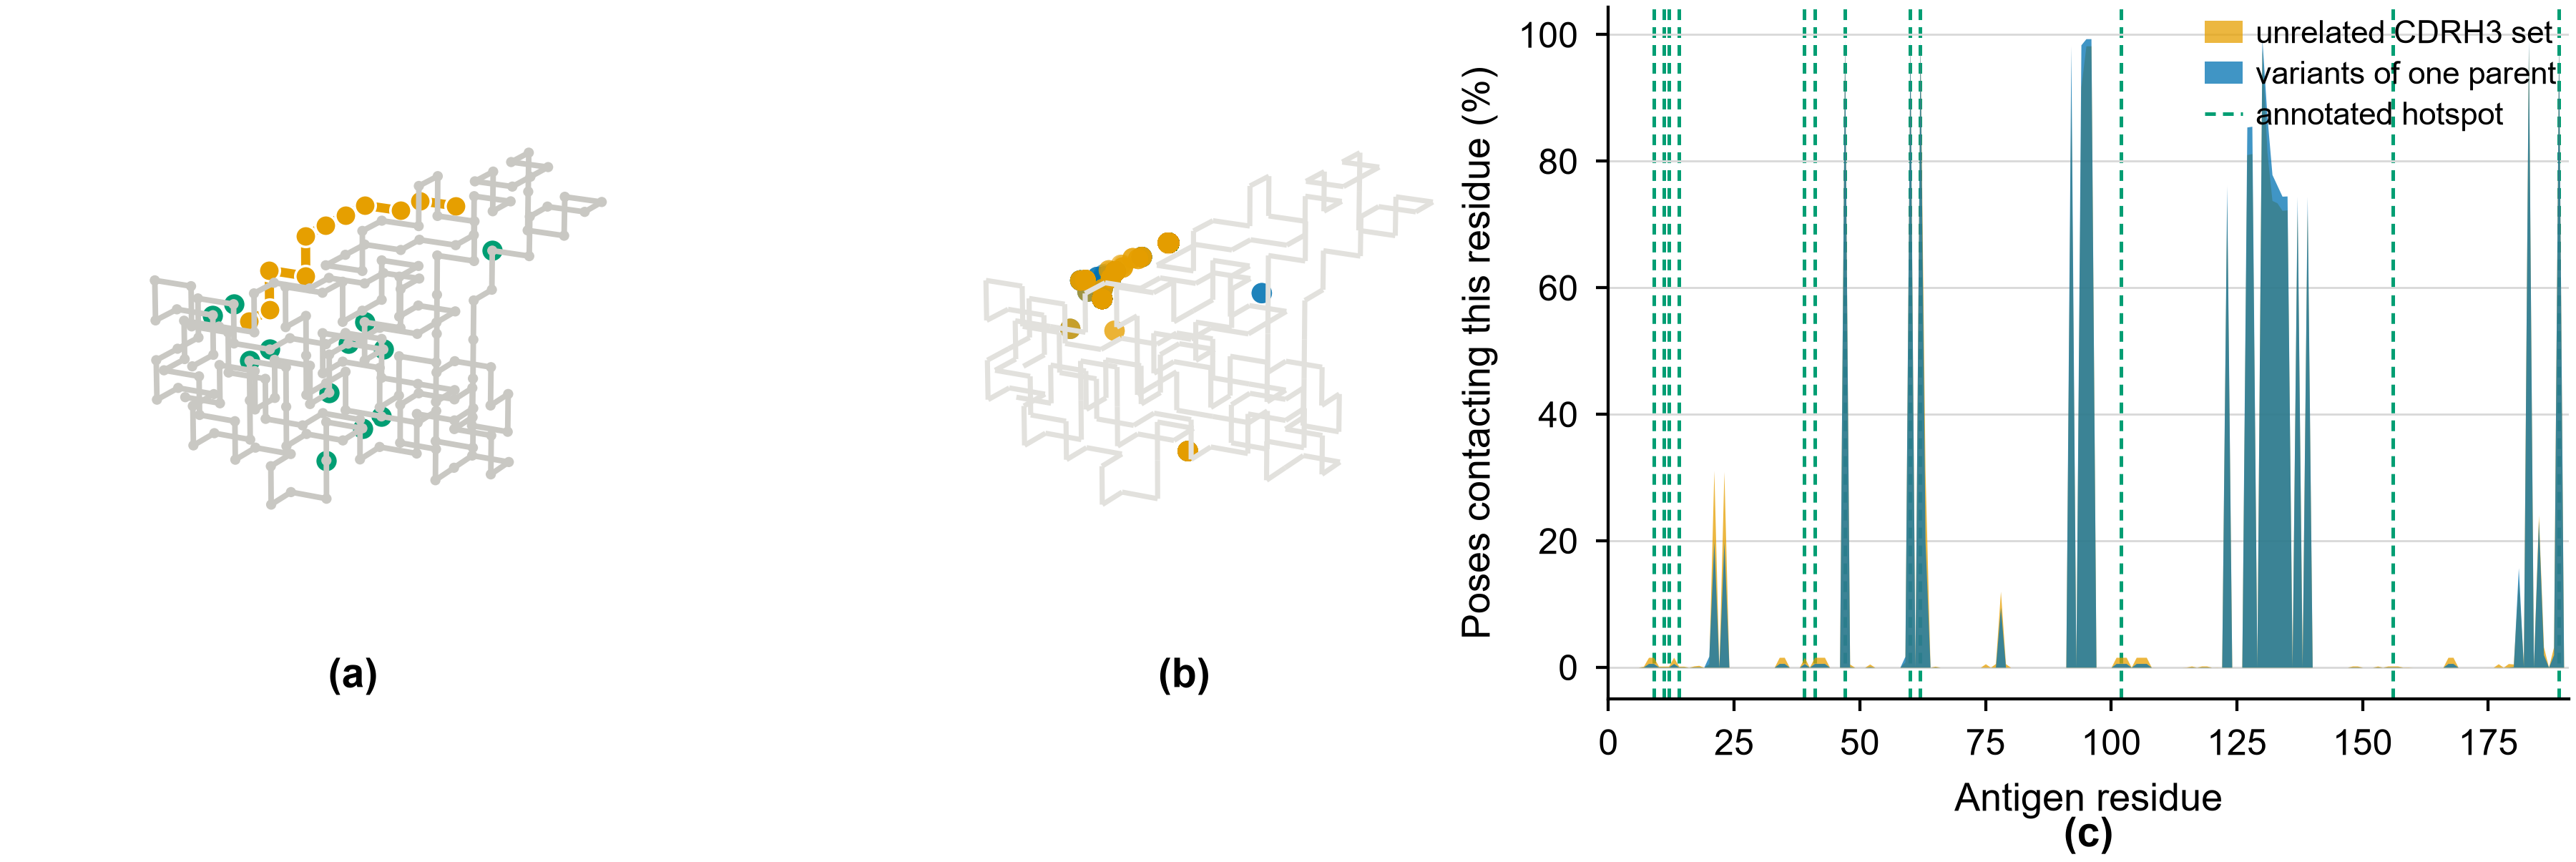
\includegraphics[width=\textwidth]{figs/F9.png}
\caption{What the oracle computes, and where the two libraries sit on it.
\textbf{(a)}, the antigen used throughout (2DD8\_S, SARS-CoV spike RBD, 192
lattice residues) in grey, with the strongest CDRH3 of the matched library
docked in orange (best energy $-126.5$) and the hotspot residues the benchmark
annotates in green. \textbf{(b)}, the centre of each pose for 700 sequences
drawn from each library, orange for the unrelated set and blue for the variants
of one parent; both clouds are tight and coincident, with a mean spread of
0.9 lattice units in each case. \textbf{(c)}, the fraction of poses contacting
each antigen residue, with the annotated hotspots dashed; 26 of 192 residues
are contacted by more than 5\% of poses in either library. The two libraries
differ in sequence space, one being unrelated CDRH3s and the other a mutational
neighbourhood of a single parent, but they reach the same face of the antigen,
so the comparison that follows changes the library without moving the binding
site.}\label{fig:design}
\end{figure}

Figure~\ref{fig:design} shows the oracle the comparison rests on: a lattice
antigen, the CDRH3 poses scored against it, and the surface each library
reaches. On the synthetic side we used the Absolut! library of 6{,}917{,}820
murine CDRH3 sequences \cite{robert2022}, drawn from observed repertoires
\cite{olsen2022}, scored against six infectious-disease antigens. On the
measured side we used AlphaSeq affinities for four targets (anti-SARS-CoV-2
VHH72, anti-TIGIT, anti-PD-1 and anti-HER2), comprising 707{,}713 measurements
\cite{engelhart2022}.

The two collections differ in five ways at once. Labels are lattice energies
versus $\log_{10} K_D$; library sizes are $6.9\times10^{6}$ versus
$2$--$3.5\times10^{4}$; the synthetic library is a set of unrelated sequences
whereas the measured libraries are mutational neighbourhoods of one parent;
CDRH3 lengths vary from 11 to 43 residues on the synthetic side but positions
are alignable on the measured side; and only the measured data carry assay
noise, which we quantified as $\sigma = 0.27$ in $\log_{10} K_D$ from 100
replicate measurements of the wild-type parent.

\subsection*{Four differences appear when conditions are not matched}

Compared as they stand, the two collections differ in four ways
(Table~\ref{tab:effects}).

\begin{table}[htbp]
\caption{The four differences that appear when the synthetic and measured
regimes are compared as they stand, and what remains of each once library size
and structure are matched. The lattice oracle is unchanged throughout; only the
library differs, except that the representation row must also change encoder,
because an aligned one-hot does not exist for a library without a parent. Both
arms of every row are measured over twenty splits or seeds with bootstrap
intervals. Search recoveries are in Supplementary Tables~S1 and~S9, the
representation comparison in Tables~S2, S7 and~S8, and the architecture
crossover in Table~S3.}\label{tab:effects}
\begin{tabular}{@{}p{2.4cm}p{2.7cm}p{3.6cm}p{1.8cm}@{}}
\toprule
Apparent effect & Unmatched comparison & After matching size and structure &
Verdict \\
\midrule
Search advantage,
active over random & 1{,}620-fold &
290 to 500 measurements to recover half the top 1\% across seven matched
lattice libraries, against 799 to over 1{,}000 across four measured targets &
Narrows, does not close \\[4pt]
Representation,
one-hot against ESM-2 & one-hot ahead at every training size,
$+0.082$ pooled over 100 train/test splits of the one unmatched library &
the language model ahead in all seven matched libraries, $-0.005$ to $-0.022$
pooled; largest at 200 labels, and by 4{,}000 one-hot is ahead in five of seven
&
Reverses, then reverts \\[4pt]
Architecture,
ridge against CNN & crossover seen only on the lattice &
crossover at 2{,}000 labels in both regimes; ridge ahead below, the network
ahead above & Agrees \\[4pt]
Learnability split,
noise against smoothness & 54\% / 46\% &
38\% / 62\%, with the two arms varying at different numbers of positions &
Not measurable \\
\botrule
\end{tabular}
\end{table}

Guided search appeared far more valuable on the synthetic side: with a budget
of 2{,}000 measurements out of $6.9\times10^{6}$, active learning recovered 378
of the 691 sequences in the top 0.01\% against 0.23 for random sampling, a
1{,}620-fold ratio, where measured data gave a threefold advantage. The
preferred representation differed, with one-hot encoding ahead of ESM-2
embeddings \cite{lin2023} at all five training-set sizes on the synthetic
library while the language model won 16 of 19 intervals on measured targets.
Repeated at the twenty splits used for the matched arm below, the advantage
survives: $+0.082$ pooled (95\% CI $+0.075$ to $+0.088$), one-hot ahead in 98
of 100 splits of that single library (Supplementary Table~S7), so the unmatched effect is real rather
than an artefact of thin replication. The preferred architecture appeared to differ
as well: ridge regression beat a max-pooling convolutional network across the
whole measured range, which stopped at 5{,}000 labels, whereas the network
overtook ridge within that range on the synthetic library. Finally, a
decomposition of the learnability gap attributed 54\% to measurement noise and
46\% to a residual we initially read as intrinsic smoothness of the lattice
energy function.

\subsection*{Two of the four disappear, one is unmeasurable, and one narrows}

We then rebuilt the synthetic library to match the structure of the measured
ones (Supplementary Figure~S2), taking a strong binder of length 17 as the
parent (\texttt{CARDRLLWLRLWYFDVW} for SARS-CoV spike RBD) and enumerating all
285 single mutants plus random doubles and triples to reach 6{,}000 sequences,
the recipe used to build the AlphaSeq libraries. Seven libraries built this way
pass the consistency check described in Methods and are used throughout. Every
sequence was scored with the same binary, so the labels remain lattice energies
from the same oracle and only library size and structure change.

Two differences resolved, one proved unmeasurable, and the fourth narrowed
without closing (Table~\ref{tab:effects}).

The search advantage collapsed by three orders of magnitude but did not reach
the measured range. Reporting it needs one preliminary. The quantity method
papers use, recovery by guided search relative to random sampling, is only
interpretable while the numerator can still rise: at a budget of 1{,}000 out of
6{,}000, five of the seven matched libraries already recover 95\% or more of
the top 1\%, so their ratios there are lower bounds rather than values. At 500
none of the seven does, and the ratio is 6.0 to 11.3-fold on the matched
lattice against 2.0 to 3.6-fold across the four measured targets subsampled to
the same size (Fig.~\ref{fig:search}a; Supplementary Table~S9, which gives four
budgets). The ranges do not overlap at 300, 500 or 1{,}000.

A quantity with no ceiling says the same thing more plainly: the number of
measurements needed to recover half the top 1\%. That is 290 to 500 on the
seven matched libraries, against 799 and 952 for two of the measured targets
and more than 1{,}000 for the other two, while random sampling reaches half in
none of the eleven within the budgets tested (Supplementary Table~S16). An
earlier pass at five seeds gave 3.3-fold against 3.0-fold at a budget of
1{,}000 and so appeared to agree; the same code at twenty seeds produces all
225 of those cells exactly, so the change is replication rather than method,
and the apparent agreement came from reading a saturated ratio. Matching
therefore accounts for three orders of magnitude and leaves a factor of two to
three.

What remains is not a property of the labels but of how learnable each library
is. The ratio tracks the held-out Spearman a ridge surrogate reaches on 1{,}000
labels from that library (Fig.~\ref{fig:search}b). Because the two regimes
separate on both axes, we test the association where it can be tested: within
the four measured targets, whose ratios do not saturate, the two quantities
order identically ($r = 1.00$, $p = 0.002$). Learnability in turn tracks the
number of varying positions: 15 in
the matched libraries against 59 to 89 in the measured ones, a difference
matching size and mutational structure does not remove. Reducing the varying
positions within a matched library, holding the antigen, the oracle, the size
and the mixture of single, double and triple mutants fixed and averaging over
randomly drawn position sets, raises held-out Spearman in all seven antigens,
by $+0.031$ on average from 15 positions to 8 (sign test $p = 0.008$;
Supplementary Table~S11). The direction is
right and the size is not: the same quantity differs by 0.2 to 0.4 between the
matched and measured arms, so dimension is one term and measurement noise,
measured separately below, is another. The more direct test, varying the
positions and re-running the search comparison, fails for a reason worth
recording: at the common subset size the budget is a quarter of the library and
the ratio saturates (Supplementary Table~S12).

\begin{figure}[htbp]
\centering
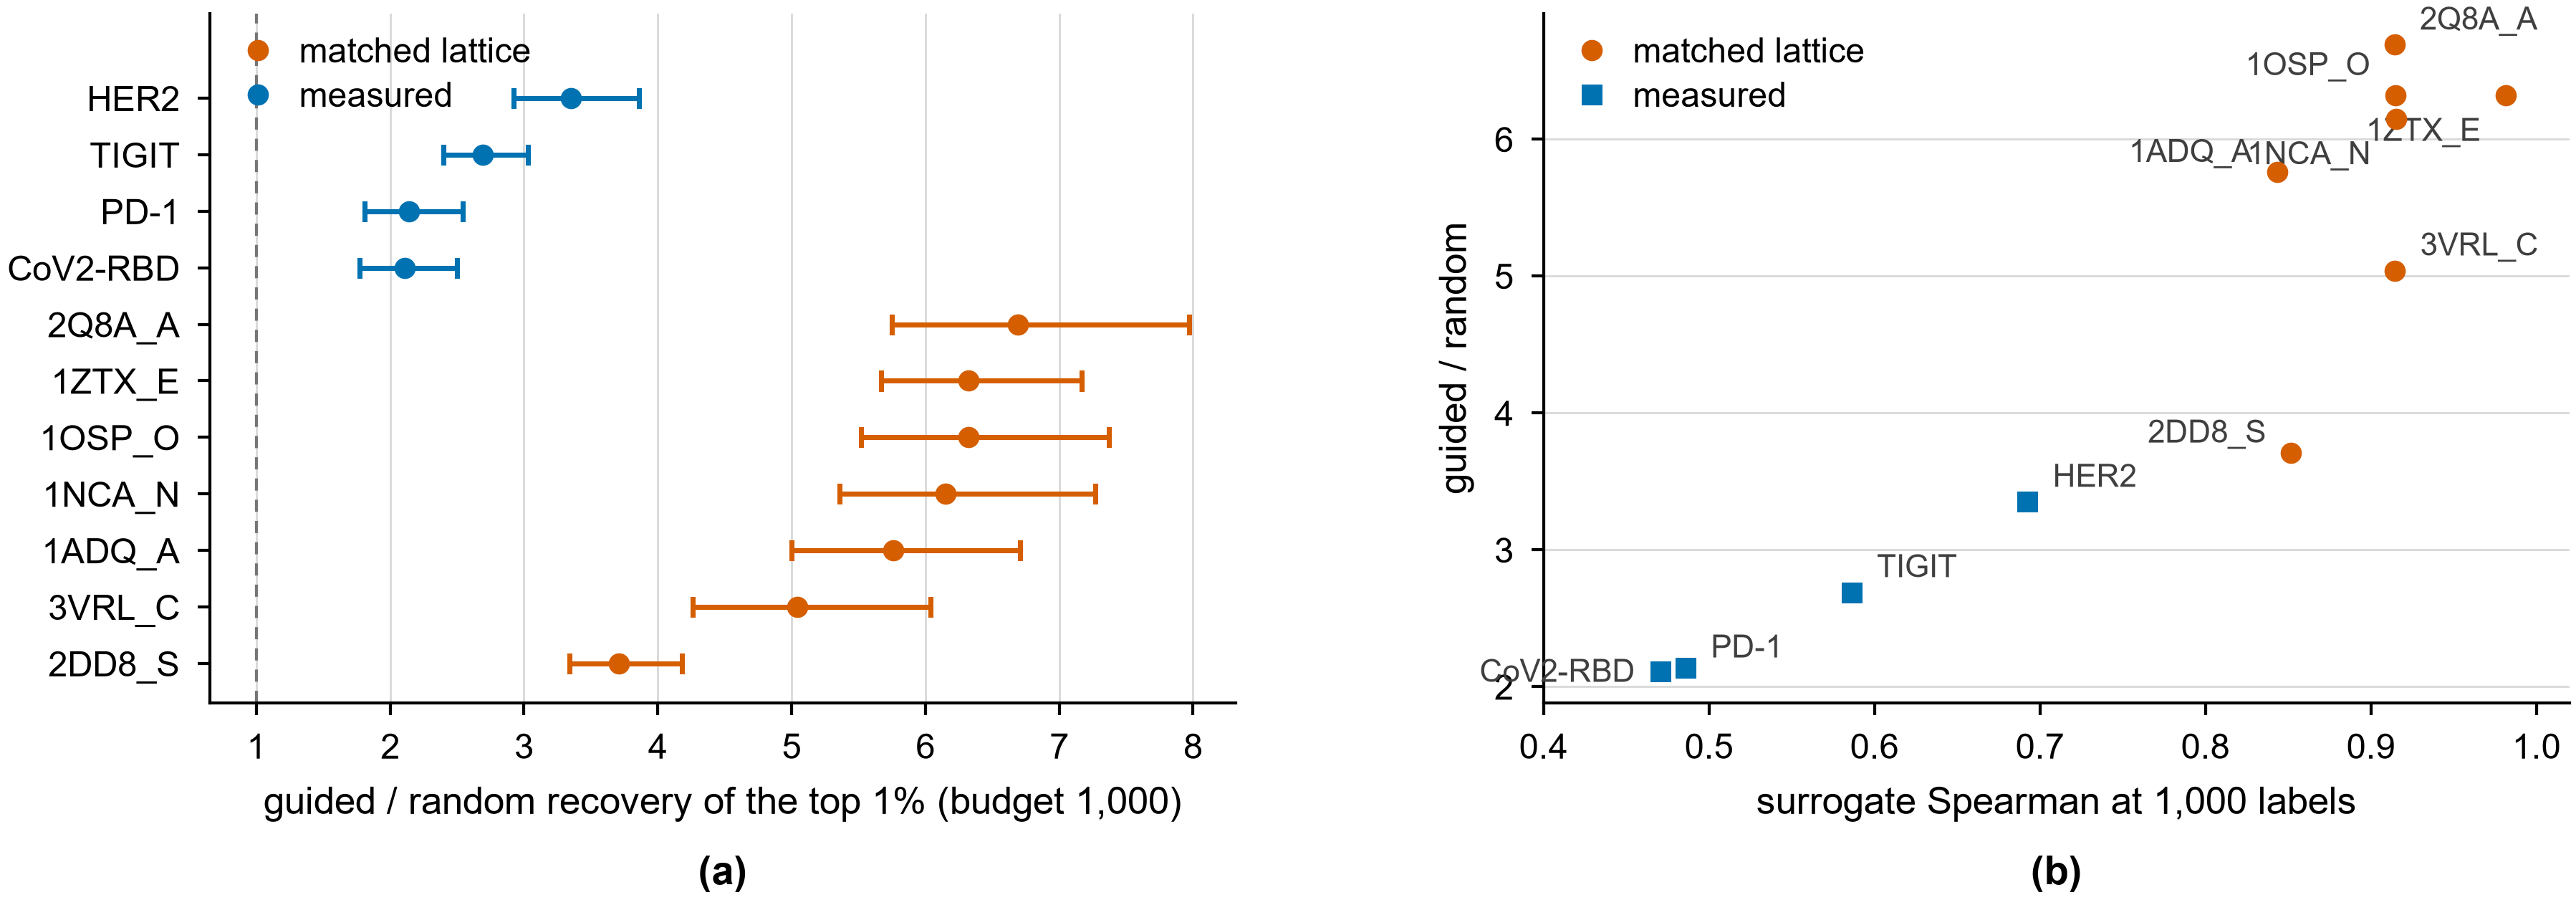
\includegraphics[width=\textwidth]{figs/F2.png}
\caption{Matching narrows the search advantage without closing it, and what
remains tracks how learnable each library is. \textbf{(a)}, recovery of the top
1\% by guided search relative to random sampling at a budget of 1{,}000 out of
6{,}000, for seven matched lattice libraries and four measured targets
subsampled to the same size. Points are ratios of mean recovery over twenty
seeds; bars are 95\% bootstrap intervals on that ratio. Only the lowest matched
library overlaps the measured range. \textbf{(b)}, the same ratios against the
held-out Spearman a ridge surrogate reaches on 1{,}000 labels from the same
library, which is itself set by how many positions vary: 15 on the matched
lattice against 59 to 89 measured. The two regimes separate on both axes, so
the correlation over all arms partly restates that separation; within the
measured targets, where nothing saturates, the ordering is exact ($r = 1.00$,
$p = 0.002$ over four targets), while within the matched libraries it cannot be
assessed because their ratios sit against the ceiling.}\label{fig:search}
\end{figure}

The representation preference reversed on the lattice itself, and did so in the
same shape for all seven matched libraries. Pooled over twenty splits and five
training sizes the mean Spearman difference ran from $-0.005$ to $-0.022$,
every interval excluding zero in favour of the language model (Supplementary
Table~S8). The shape matters more than the pooled value. The advantage is
largest at 200 labels, between $-0.031$ and $-0.083$, and it does not merely
shrink as labels accumulate but reverses: at 4{,}000 one-hot is ahead in five of
the seven libraries, one still favours the language model and one is
indistinguishable from zero, at a tenth of the magnitude seen at 200
(Supplementary Figure~S3). Which representation is preferred is therefore a
question about the label budget as much as about the library. Before matching
the dependence runs the other way: one-hot is ahead at every size and its lead
widens with training data, from $+0.037$ at 200 labels to
$+0.117$ at 4{,}000. The oracle, the scoring function and the model code are
unchanged between the two arms, but the encoders are not, and cannot be: an
aligned one-hot exists only where the library has a parent and a common length
(Supplementary Methods). The reversal therefore follows the alignability of the
library rather than the synthetic labels, with the caveat that alignability and
encoder change together and this design cannot separate them. It does not depend on which parent the
library is built around: rebuilding one library around the strongest length-17
binder instead of the one we used, which ranks 4th, leaves the direction
unchanged at every training size, though the advantage then persists at 4{,}000
labels instead of closing (Supplementary Table~S14).

The architecture crossover was not a difference between regimes but an artefact
of the range examined. Extending the measured arm from 5{,}000 to 20{,}000
training labels using the AlphaBind fine-tuning splits \cite{alphabind2025},
over twelve splits for each of three targets, located the crossover at 2{,}000
labels: ridge was ahead below it and the convolutional network above it, with
all six differences surviving Holm correction and 2{,}000 the only size at
which the two were indistinguishable (Holm-adjusted $p = 0.51$). The same
ordering holds on the synthetic library, so what had looked like a disagreement
about architecture was a disagreement about where each study stopped looking.

The learnability decomposition proved not to be measurable with these data.
Repeating it on the matched library changed the split from 54/46 to 38/62,
and the matched lattice library varies at 15 positions, of which 11 carry
signal, against 59--89 for the measured single-chain variable fragments, so the
two arms remain dimensionally unmatched. We therefore report this decomposition as
undetermined rather than quoting either value.

\subsection*{Effects that survive matching}

Two findings concern the evaluation protocol rather than the library, and
matching leaves both intact. A third is that at a budget of 200 out of 6{,}000
neither guided strategy improved on random sampling in either regime, a floor
below which the surrogate carries no information.

\textbf{Measurement noise alone costs 0.105 in Spearman.} Adding Gaussian noise
matched to the measured noise-to-signal ratio (0.424) to the matched lattice
labels reduced Spearman by 0.095 to 0.116 across training-set sizes. Because
this comparison is made within one dataset with structure held fixed, it is not
subject to the confound above.

\textbf{Random splits overstate prospective performance 6.7- to 8.1-fold}
(Fig.~\ref{fig:prospective}). On the AlphaSeq coronavirus panel a random forest
evaluated by random split recovered 40.3\% of the true top 100 within its top
500; trained on one design campaign and tested on sequences designed later it
recovered 5.0\%, an 8.1-fold loss, and ridge gives 44.3\% against 6.6\%.
Batch effects do not explain it: wild-type replicates measured in both
campaigns shifted by $+0.037$ with inconsistent sign, and Spearman is invariant
to monotone shifts. The cause is in the sequences. The first campaign stayed
near the parent, at a median of 4 mutations, whereas the second reached a
median of 9 (Fig.~\ref{fig:prospective}c), and the two separate along the first
principal component of the encoding (Kolmogorov--Smirnov $D = 0.75$). A model
fitted to the first is asked to extrapolate; random splits never pose that
question.

\begin{figure}[htbp]
\centering
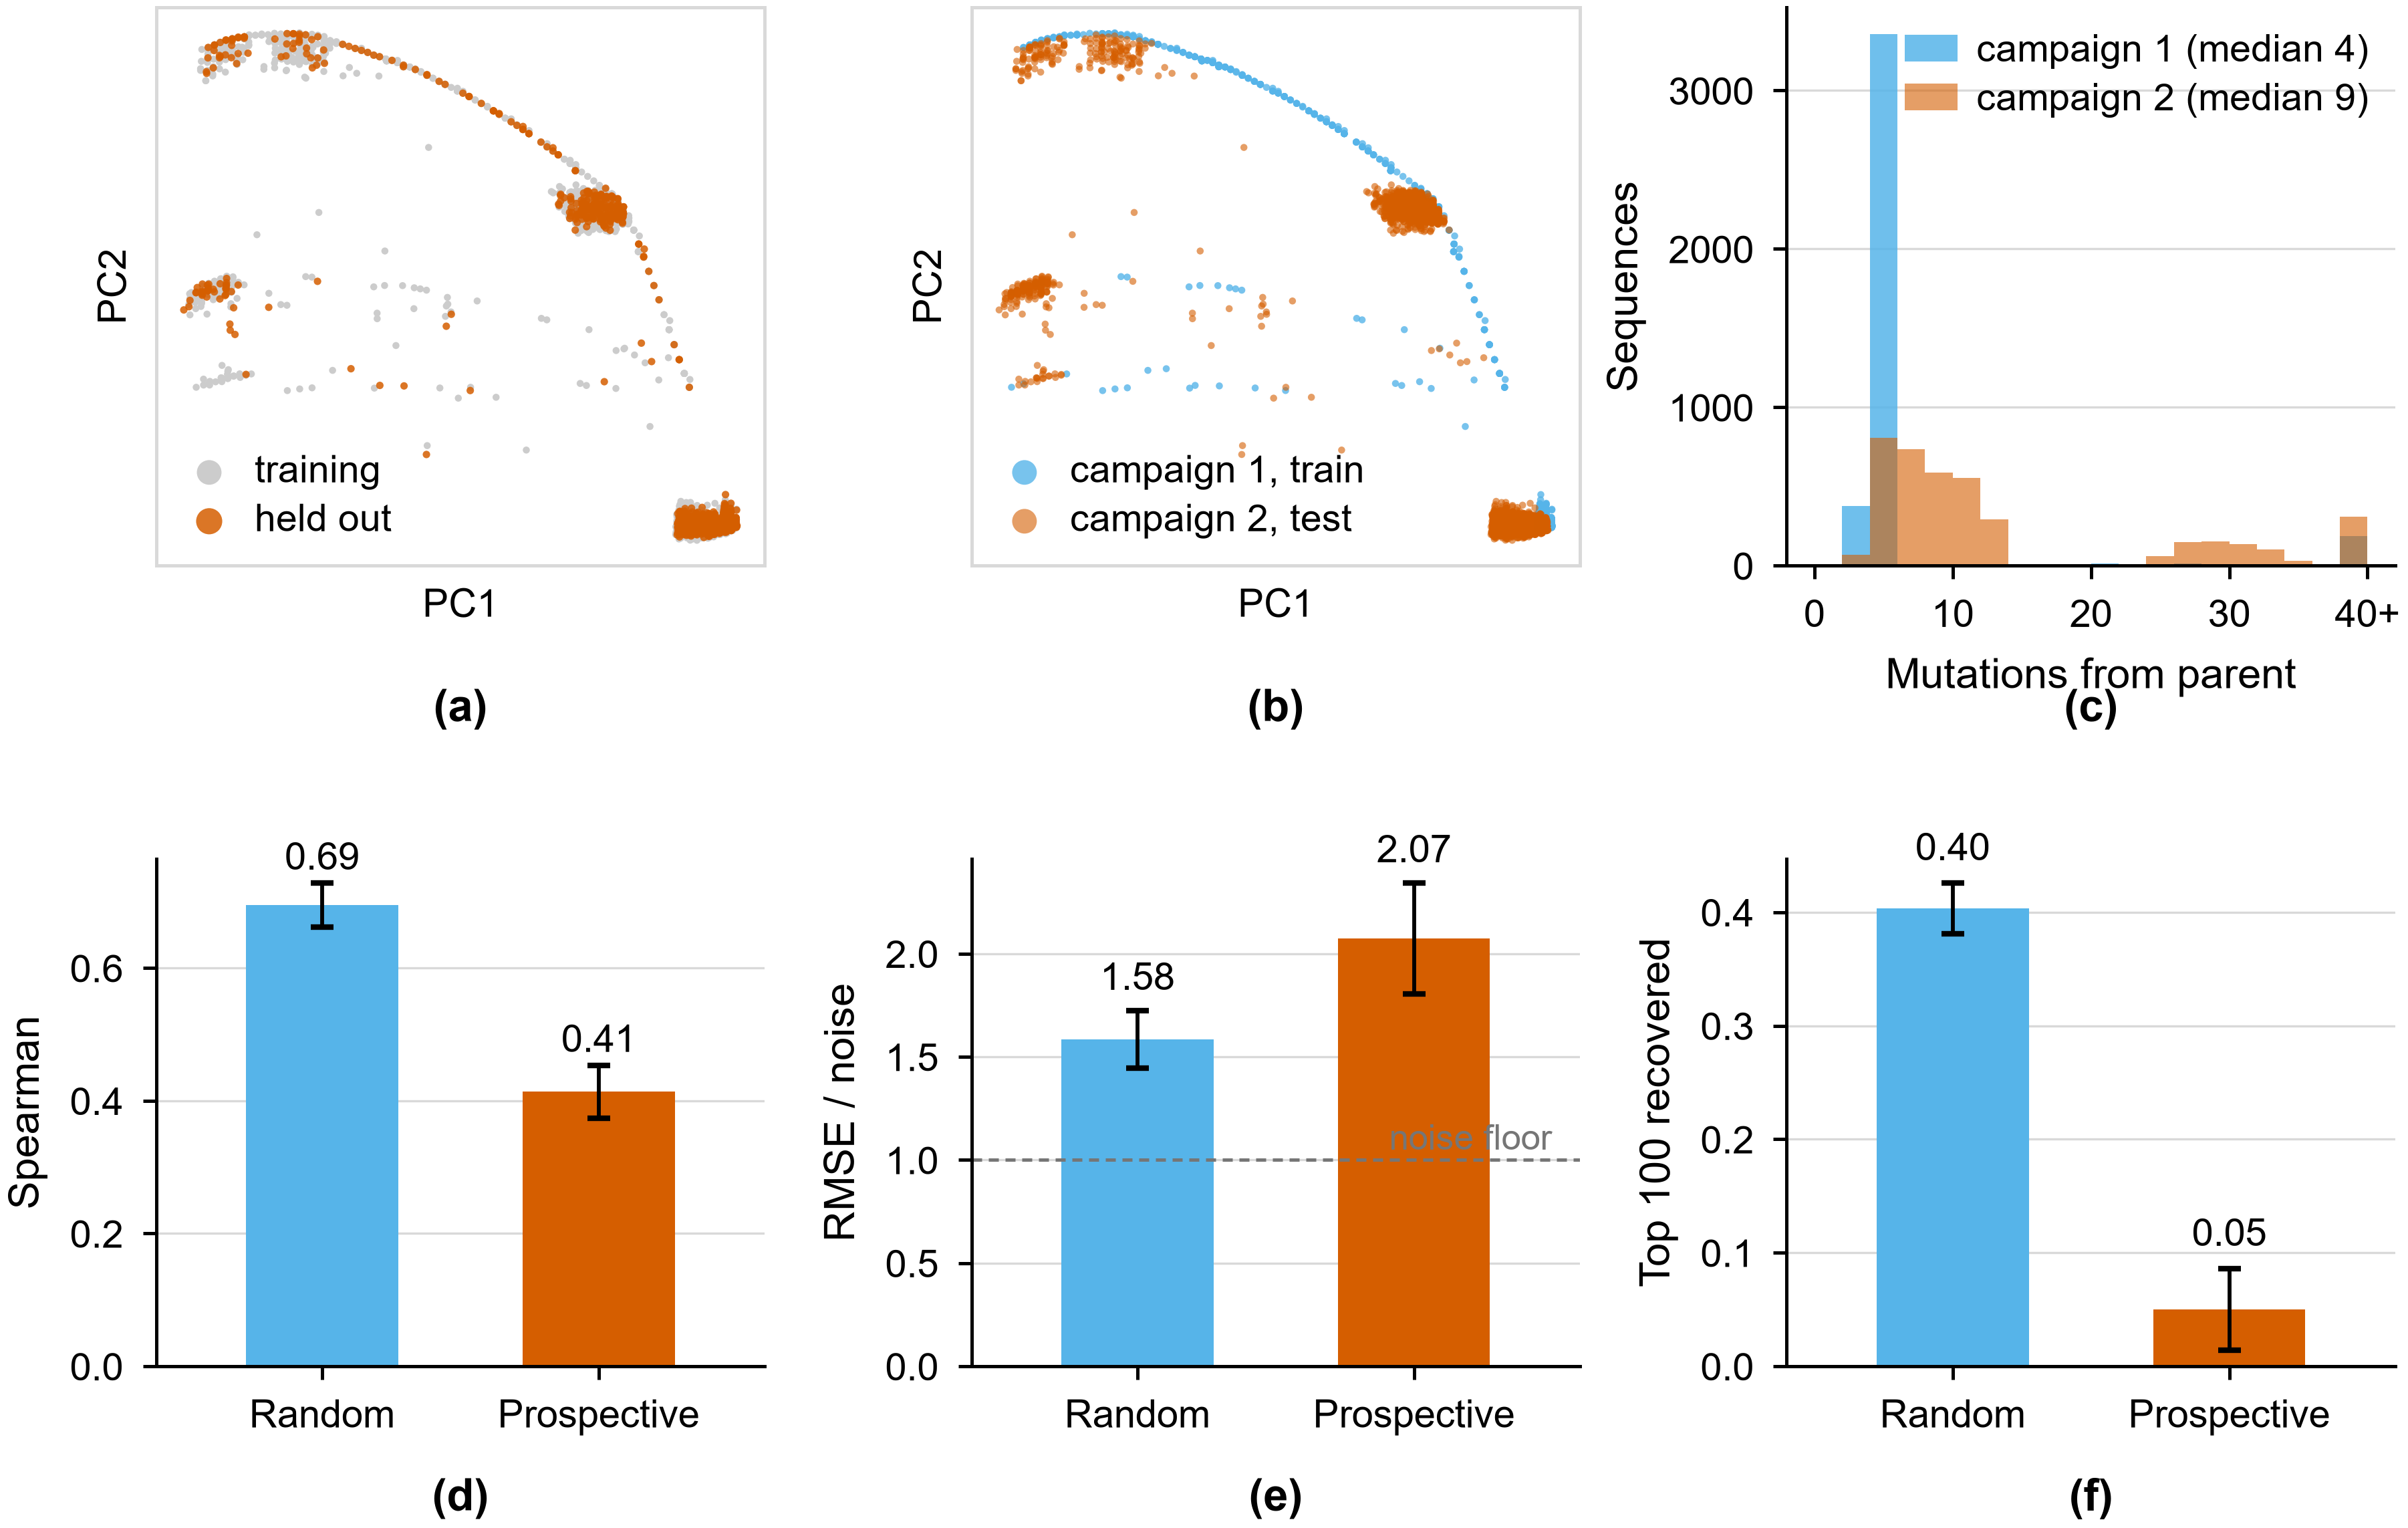
\includegraphics[width=\textwidth]{figs/F4.png}
\caption{Random splits overstate prospective performance, and why.
\textbf{(a)}, under a random split the held-out sequences lie among the training
sequences. \textbf{(b)}, under a prospective split the test set is a displaced
cloud; coordinates are the first two principal components of the one-hot
encoded sequences. \textbf{(c)}, the source of the displacement: the second
campaign designed sequences far further from the parent antibody than the
first. \textbf{(d)}--\textbf{(f)}, the cost. The same model recovers 8.1-fold less
of the true top 100 when evaluated prospectively, and a ridge regression
6.7-fold less. The measurement noise floor
was estimated from 100 wild-type replicates.}\label{fig:prospective}
\end{figure}

\textbf{Read-count models do not beat a trivial baseline on panning data}
(Supplementary Fig.~S1). On a five-round c-Met campaign \cite{yoo2020}, a
random forest predicting final-round abundance from early rounds reached AUROC
0.992 against 0.997 for simply ranking by the last available round. Sequence
alone identified the top 1\% of enriched clonotypes at 0.811 against a
permutation null of $0.482 \pm 0.056$ ($z = 5.9$), so the value of learning
lies in scoring sequences that were never measured.

\textbf{Combined representations rank highest among seven models.} The four
measured targets do not all reach the same training-set size, so we compare at
2{,}000 labels, the largest at which all four are present. Ridge on ESM-2
embeddings combined with one-hot features reached Spearman 0.648 (95\% CI
0.584--0.716), ahead of ESM alone (0.639), one-hot alone (0.626), the
convolutional network (0.576), random forest (0.533), boosted trees (0.526) and
a $k$-nearest-neighbour control (0.328) (Supplementary Figure~S4; Supplementary
Table~S5); the top three keep that order at 5{,}000 and 10{,}000 labels on the
three targets that reach them.

\subsection*{An independent prospective campaign agrees}

\begin{figure}[htbp]
\centering
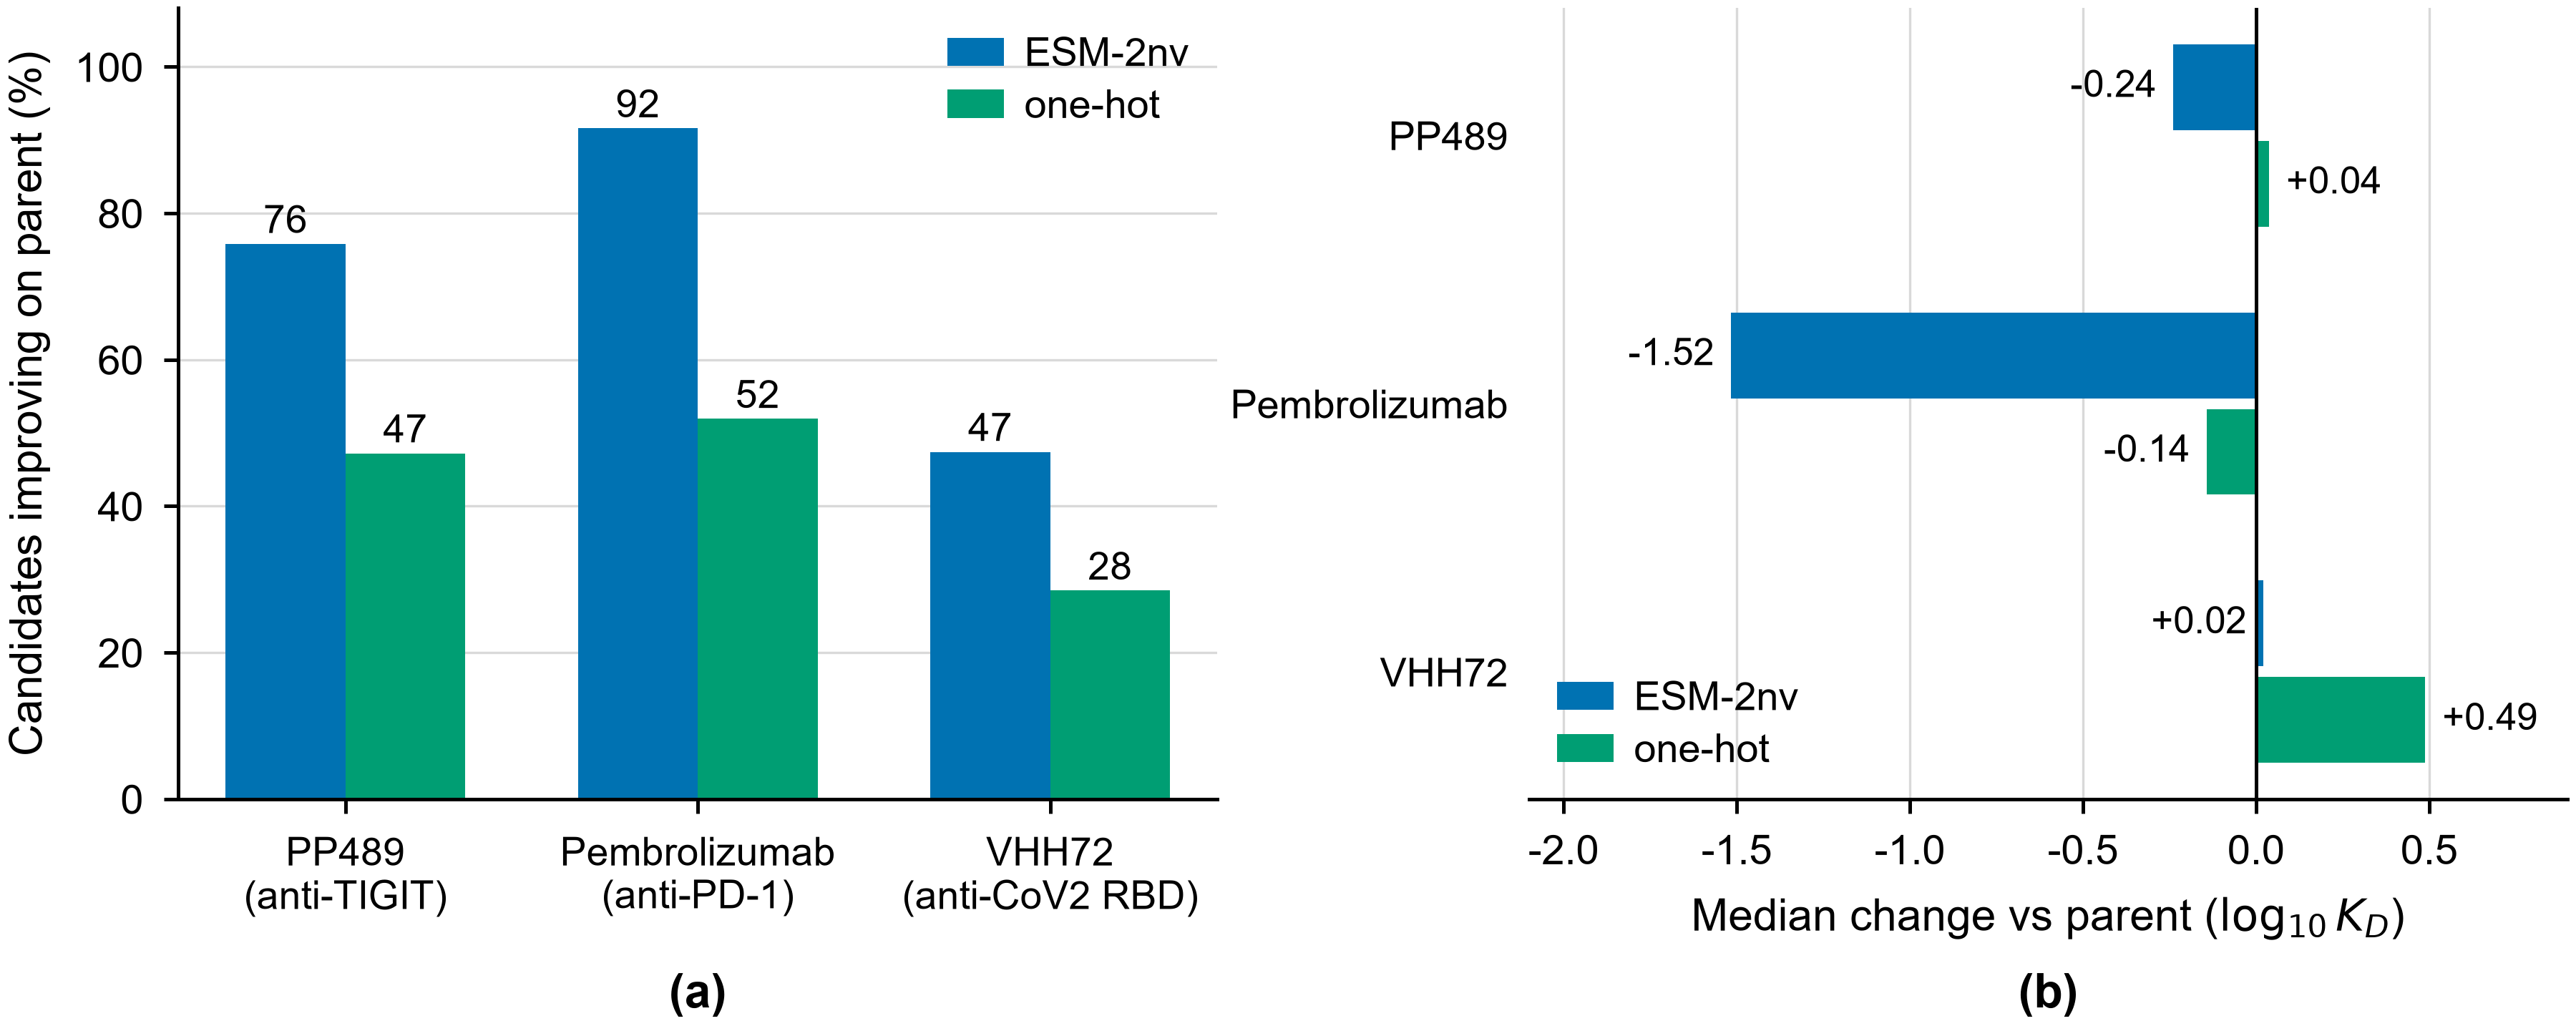
\includegraphics[width=\textwidth]{figs/F6.png}
\caption{An independent prospective campaign agrees. Candidates from
generators differing only in featurisation were all measured by AlphaSeq.
\textbf{(a)}, the fraction of candidates that improved on the parent antibody.
\textbf{(b)}, the median change in affinity, where negative values are
improvements. The language model is ahead on both measures for all three
parental antibodies.}\label{fig:external}
\end{figure}

A-Alpha Bio released the candidates proposed during the AlphaBind campaign with
the AlphaSeq measurement of each \cite{alphabind2025}. Because the generators
differ only in featurisation (one-hot against ESM-2nv embeddings), these
119{,}828 measurements are a prospective, wet-lab test of the representation
question by an independent group. The language model produced better candidates
for all three parental antibodies (Fig.~\ref{fig:external}): 76\% against 47\%
of candidates improved on the parent for anti-TIGIT, 92\% against 52\% for
pembrolizumab and 47\% against 28\% for VHH72 ($p < 10^{-249}$ in all six
comparisons; Supplementary Table~S4). These candidates are mutational
libraries, so the direction agrees with our matched-library result.

We note that the correlation between each model's own predicted affinity and
the subsequent measurement is strongly attenuated in this dataset, because
candidates were selected to have similar predicted values; predicted values
have 0.16 times the standard deviation of the measurements. We therefore do
not interpret that correlation.

\section*{Discussion}\label{sec:discussion}

Two of the four differences we examined were properties of library size and
structure rather than of the synthetic labels, and a third could not be
measured once the arms were comparable. The fourth, the search advantage, fell
by three orders of magnitude and stopped short of the measured range. Read
positively, Absolut! is a useful proxy: at matched size and structure it gave
the same answers as measured data for the representation choice and the
architecture crossover, and brought a 1{,}620-fold search advantage into
single digits. The difficulty lies in comparisons varying several factors at
once.

The residue is itself informative. Guided search still works better on the
matched lattice than on any measured target, and how much better tracks how
well a simple surrogate fits each library rather than anything about the
labels. That tracks the number of varying positions, which matching leaves
untouched. Narrowing the design space inside a matched library
reproduces the direction of the effect but about a tenth of its size, so
dimension is one term and measurement noise, measured separately at 0.105
Spearman, presumably another. We claim no complete decomposition, only that
what survives matching has a measurable correlate, and that it is not the
label source.

That positive reading has a boundary, which the cognate-antibody test locates.
Across 88 antigens the oracle did not place a known binder above sequences with
no known affinity for it, and no antibody identified its own antigen. Two
observations explain why. The preferred contact site is a property of the
discretised antigen, so sequences that differ completely are scored in the same
pocket; and the energies themselves correlate across antigens, so changing the
antigen barely reorders the good sequences. The lattice is a consistent ranking
function over sequences, not a model of which antibody binds which antigen.
That suffices for comparing methods under a fixed and reproducible label
source; it does not license reading a high lattice energy as evidence of
binding.

This has a practical consequence. Before selecting a method on a synthetic
benchmark, we suggest matching five properties to the intended application:
library size; library structure, meaning a mutational neighbourhood or
unrelated sequences; the number of varying positions, which our results
identify as the one that survives matching the first two; measurement noise, at
the noise-to-signal ratio of the intended assay; and the range of training-set
sizes. Reporting these alongside benchmark results would make cross-study
comparison interpretable.

Which of the five matter most depends on what the benchmark is being asked.
For an early screen, where a few hundred labels are affordable and the question
is which model family to build on, a synthetic benchmark is a reasonable guide
even unmatched: method rankings agreed at $+0.96$ at 200 labels. For selecting
among methods at the budgets an affinity-maturation campaign actually reaches,
a thousand labels and upwards, the agreement had fallen to $+0.64$ and the
leading model differed, so the choice should be made on measured data or on a
library matched in the number of varying positions. For estimating how many
measurements a campaign will need, the matched lattice is optimistic by roughly
a factor of two even after matching, and the number to report is measurements
to a stated recovery rather than a ratio over random sampling, which saturates.
And where the question is whether a sequence binds at all, rather than which
method ranks it best, the lattice should not be used as evidence: it separates
antigens only among the strongest binders it scores, and real antibodies are
not scored there.

The effects that survived matching concern the evaluation protocol rather than
the model. The noise floor was measured within one dataset and argues for
reporting error relative to assay noise rather than in absolute units. Random
splits overstated prospective recovery 8.1-fold because the second design
campaign explored much further from the parent, so a model fitted to the first
is asked to extrapolate; retrospective accuracy on a mutational neighbourhood
says little about the next round of designs, a gap that iterative and
uncertainty-aware methods are built to address \cite{hie2020,settles2009}. The panning re-analysis points the same way, and throughout, the
nearest-neighbour control separated clearly from every model, the minimal
evidence that a comparison measures learning rather than composition
\cite{chuang2018}.

These findings are consistent with the transferability originally reported for
Absolut! \cite{robert2022} and sit alongside a broader result in protein
engineering, that how a training set is designed often matters more than which
model is fitted to it \cite{wittmann2021,biswas2021,yang2019}. What we add is
that this applies to the benchmark as much as to the campaign.

We are not aware of a published conclusion that these results overturn, and we
make no such claim: the applications we know of either state their own limits
on transfer or work in a setting the confound does not reach, such as de novo
design rather than selection from a library \cite{akbar2022,khan2023}. The
contribution is preventive. The comparison that would be misled is easy to set
up, costs nothing to control once the factors are named, and the quantities
above say how large the error would be.

Several limitations bound what we can claim. We performed no wet-lab
experiments; all measured data are third-party. Each matched library varies at
15 positions, of which only 11 carry signal because the oracle scores the best
11-mer slice, so against 59--89 in the measured fragments the dimensional
mismatch is reduced but not eliminated, and seven antigens cannot speak for the
159 in the collection. The first library we built for one of them was written
by a scoring run that failed without raising an error, and had we not checked
it against the released table we would have reported the opposite conclusion
about representations, in the direction that supports our own argument
(Supplementary Table~S10); the check, not our judgement, caught it. Our
intervals resample train/test splits, so they capture variability due to the
split but not due to which sequences the library happens to contain.

The cognate-antibody test is bounded differently, because an absence of signal
is bounded by the sensitivity of the instrument. We therefore measured that
sensitivity: lowering every cognate energy by a fixed amount, the sign test
reaches 95\% power at 3 energy units and the Kolmogorov--Smirnov test 97\% at
2, against a library whose energies span $-131$ to $-75$ (Supplementary
Table~S13). An effect of that size would have been seen, so the absence is not
one of resolution.

A power calculation bounds the test from inside its own assumptions, so we also
ran it on sequences that are binders by construction. For each of six antigens
we drew two arms that share the antigen, the CDRH3 length and the mutational
neighbourhood structure and differ only in strength: a strong arm from the
matched library, whose members the oracle ranks in its top percentile, and a
weak arm from the neighbourhood of a parent at the 45th energy percentile,
where the native cognate antibodies sit. Holding the other axes fixed is what
licenses reading the difference as an effect of strength. The strong arms
placed the home antigen consistently ahead, at a median normalised rank of
0.092 to 0.326 against a chance value of 0.5, and within every one of the
twelve arms a sequence's own rank tracked its energy percentile (Spearman
$+0.32$ to $+0.91$, $p < 0.002$ in all twelve). In the weak arms the effect
weakened sharply or vanished, to 0.152--0.761, and it did so in all six
antigens (two-sided exact $p = 0.031$; Supplementary Tables~S18 and~S19).

The test therefore has sensitivity to very strong lattice binders, but in the
weak range the native antibodies occupy that sensitivity falls away, and by
different amounts in different antigens: one antigen retains a median rank of
0.152 while another reaches 0.761. We state this as a bound on the evidence
rather than as a property of the oracle, because the two cannot be separated
here. The weak-arm sequences are not known binders, so a weak pairing signal
that the test cannot resolve and an oracle that carries no such signal at that
strength would look the same. What remains is that at the strength real
antibodies occupy, this benchmark does not distinguish which antibody binds
which antigen. The test also scores CDRH3 alone, without the light chain and
the five other loops, against an antigen reduced to a lattice; whether a richer
encoding would recover the pairing is open.

Two directions follow. The first is to continue the matched construction across
the collection, which is inexpensive because the oracle runs on any sequence.
The second is prospective: the checklist predicts which methods transfer, and
that is testable in a campaign reporting a held-out round. Neither requires a
new model, which is the useful implication of this work: much of the apparent
disagreement between synthetic and measured evidence is a property of how the
comparison was set up, and is fixable by design rather than by better methods.

\section*{Methods}\label{sec:methods}

\subsection*{Data}

Absolut! binding energies for six antigens (2DD8\_S, 1NCA\_N, 1ZTX\_E,
1OSP\_O, 2Q8A\_A, 3VRL\_C) were obtained from the project archive and reduced
to one energy per CDRH3 by retaining the best-scoring 11-mer slice, giving
6{,}917{,}820 sequences common to all six; a seventh, 1ADQ\_A, was added
later for its matched library alone. Measured affinities, obtained by the
yeast-mating AlphaSeq assay \cite{younger2017}, were taken from the
open-alphaseq release \cite{engelhart2022}; we retained pairs with a
reported affinity, sufficient replicate observations and above-background
binding, and averaged replicates. The AlphaBind campaign data and its
fine-tuning and validation splits were obtained from the accompanying
repository \cite{alphabind2025}. Panning reads for BioProject PRJNA607865 were
downloaded from the European Nucleotide Archive; CDR3 sequences were extracted
by translating both mates in three frames and matching the conserved framework
anchors, recovering CDR3 from 86--92\% of reads. One run (VL round 1) was
excluded because only 5.1\% of its reads carried a recognisable CDR3.

\subsection*{Matched libraries}

The Absolut! source was compiled from the public repository; on Windows the
binary crashed while processing structure files, so all scoring was performed
under Linux. Precomputed structures were downloaded per antigen and the
interaction profiles regenerated locally. Matched libraries
were built by selecting a parent CDRH3 of length 17 among the lowest-energy for
that antigen, enumerating all 285 single mutants at the 15 non-terminal
positions, and adding deduplicated random double and triple mutants, drawn
with probability 0.6 and 0.4, until 6{,}000 unique sequences were reached. For SARS-CoV spike RBD the parent
(\texttt{CARDRLLWLRLWYFDVW}, $-121.84$) ranks 4th of the 748{,}021 length-17
sequences in the published table, the lowest being $-125.07$; we state the rank
rather than call it the minimum, because the two differ and the distinction is
checkable against the released data. Sequences were scored
in \texttt{repertoire} mode and the best slice per sequence retained.

Each library was then checked against the released one. The parent appears in
both, and because the same binary, antigen and scoring function produced them,
its energy must agree. Since the two libraries otherwise overlap only by
chance, we also rescored 340 published sequences per antigen, spanning both
tails and all lengths. All 2{,}380 agreed to within $3.7\times10^{-6}$, the
rounding of the released table's single-precision energies; the tolerance is
$10^{-3}$ (Supplementary Table~S17).

The check is worth stating because it caught one. The first library built for
influenza N9 neuraminidase disagreed by 13.15 energy units; its scoring run had
written output after failing, and the failure was discarded rather than raised.
The wrapper was changed to raise on a non-zero exit, the library was rebuilt,
and it now agrees to $1.5\times10^{-6}$. The two versions differ for 5{,}909 of
6{,}000 sequences by a median of 7.0 energy units, and analysing the first would
have reversed the representation result (Supplementary Table~S10). Seven
libraries pass and are used throughout.

\subsection*{Models and features}

The two library types require different encoders, and this is a property of the
libraries rather than a choice: a mutational neighbourhood admits an aligned
one-hot encoding and the released library, which has no parent and lengths from
11 to 43, does not. Both encoders and the ESM-2 settings are given in
Supplementary Methods. Because the encoders are not interchangeable, a
comparison of representations between the two arms confounds the encoder with
the library, which is one reason the matched arm is the one that carries the
claim. Seven models were compared:
ridge regression on one-hot
features; histogram gradient boosting and random forest on ordinal tokens;
$k$-nearest neighbours ($k = 10$) on Hamming distance as a triviality control;
a convolutional network with an embedding layer, two convolutional layers and
global max pooling, whose pooling mirrors the best-slice rule of the lattice
oracle; ridge on per-position ESM-2 (35M) embeddings reduced to 48 principal
components; and ridge on the concatenation of the last two. Language-model
embeddings were mean-pooled over the whole sequence in an initial analysis and
taken per varying position thereafter, as whole-sequence pooling averages away
the few positions that distinguish members of a mutational library.

Ridge regularisation was set to $\alpha = 1$ for one-hot features and
$\alpha = 50$ for the higher-dimensional embedding features, values chosen once
on a held-out fold of a single target and then held fixed for every experiment
reported here, so that no comparison benefits from per-arm tuning. The
convolutional network used a 32-dimensional embedding, 96 channels, and a fixed
budget of approximately 4{,}000 gradient steps at batch size 128, with targets
standardised to zero mean and unit variance; this budget rather than a fixed
epoch count keeps optimisation effort comparable across training-set sizes.
Boosted trees and random forests used the library defaults with 200 estimators
and a minimum leaf size of two.

\subsection*{Evaluation}

Training-set sizes of 200 to 20{,}000 were drawn from a held-out permutation
with 1{,}500--5{,}000 sequences reserved for testing. Exploratory sweeps used
three to five splits; every comparison on which a claim rests was then repeated
at twenty splits for the representation question and twelve for the
architecture question, and the matched and unmatched arms of the representation
comparison use the same twenty splits, the same training sizes, the same models
and the same random seeds, so that the two can be placed side by side. We
report Spearman rank correlation and the fraction of the true top 100 recovered
within a model's top 500. Two different bootstrap units appear and the
distinction matters: where several measured targets are available, intervals
resample targets rather than individual predictions, because nested subsets of
one dataset are not independent observations; within a single library, where
there is one target, they resample the splits. Both are percentile bootstraps
over 10{,}000 resamples.

\subsection*{Search experiments}

Search proceeded in two stages: a sparse ridge model scored the entire library,
and the convolutional network reranked its top 200{,}000. Three strategies were
compared at equal budget: uniform random sampling; a single-shot strategy that
spends an initial quarter of the budget at random, fits once and selects the
remainder; and active learning, which spends the remaining budget over three
rounds with 20\% held for exploration. We report recovery of the top 0.01\% or
top 1\% depending on library size, the best value found, and the gap to the
library optimum.

\subsection*{Statistics}

The independent unit is the antigen. Seven matched libraries were built,
and every quantity reported across libraries is summarised over those seven.
Within one library, repeated train/test splits and random seeds estimate the
uncertainty of that library's value; they are not treated as independent
observations and are never pooled across libraries as though they were. Where
a test is reported over antigens, its $n$ is the number of antigens.

The two comparisons that the text states as directional claims (one-hot
against the language model on the matched library, and ridge against the
convolutional network on measured targets) were each repeated over twenty and
twelve independent train/test splits respectively, rather than the three to
five used for the exploratory sweeps. At each training size the paired
difference in Spearman correlation was tested against zero by a one-sample
$t$-test across splits, with the sign confirmed by a Wilcoxon signed-rank test,
and summarised by a percentile bootstrap over 10{,}000 resamples of the splits.

Because each comparison is swept over training sizes, the sweep forms a family
of tests and the smallest $p$-value in it would overstate the evidence if
quoted alone. Each family was therefore corrected by the Holm--Bonferroni
procedure \cite{holm1979}, controlling the family-wise error rate, and separately
by the Benjamini--Hochberg procedure \cite{benjamini1995}, controlling the false
discovery rate; both
adjusted values are reported in Supplementary Table S2. Families were corrected
separately rather than pooled, since they address distinct questions and
pooling would penalise each for the breadth of the others.

Splits are independent partitions of one library, so these intervals describe
variability due to the train/test split and to model initialisation. They do
not describe variability due to which sequences the library contains, which
would require independently constructed libraries; the matched-library results
therefore rest on a single antigen and should be read as such.

\backmatter

\bmhead{Supplementary information}

Supplementary Table S1 lists every quantity reported in this article together
with the source file and the computation that produced it. Supplementary
Table S2 gives the raw, Holm--Bonferroni-adjusted and
Benjamini--Hochberg-adjusted $p$-values for every family of tests, with the
effect size beside each. Supplementary Figure S1 reports the
re-analysis of the panning campaign. Supplementary Data comprise the matched library generated here and the
per-experiment result tables underlying every figure.

\bmhead{Acknowledgements}

This work was supported by the Culture, Sports and
Tourism R\&D Program through the Korea Creative Content Agency grant funded by
the Ministry of Culture, Sports and Tourism in 2024 (RS-2024-00398310). This
work was supported by internal fund/grant of Electronics and
Telecommunications Research Institute (25YT1400). We thank the authors of
Absolut!, open-alphaseq and AlphaBind for releasing the data and code that
made this re-analysis possible.

\section*{Declarations}

\begin{itemize}
\item \textbf{Funding.} This work was supported by the Culture, Sports and
Tourism R\&D Program through the Korea Creative Content Agency grant funded by
the Ministry of Culture, Sports and Tourism in 2024 (RS-2024-00398310). This
work was supported by internal fund/grant of Electronics and
Telecommunications Research Institute (25YT1400).
\item \textbf{Competing interests.} The authors declare no competing interests.
\item \textbf{Author contributions.} D.K. conceived and designed the
study, performed the analyses, wrote the manuscript, administered the project
and acquired funding. M.B. contributed to the methodology, to the validation
of the results and to data curation, and revised the manuscript. Both authors
read and approved the final manuscript.
\item \textbf{Data availability.} Every primary dataset analysed here is
third-party and already public: Absolut! lattice binding energies
(\url{https://greifflab.org/absolut/}); open-alphaseq AlphaSeq affinity
measurements
(\url{https://huggingface.co/datasets/aalphabio/open-alphaseq}); the AlphaBind
campaign measurements (\url{https://github.com/A-Alpha-Bio/alphabind}); the
c-Met panning reads deposited under BioProject PRJNA607865. The analysis
outputs generated in this work are archived at Zenodo
(\url{https://doi.org/ZENODO-DOI-PENDING}): the per-experiment result tables
from which every figure and every quantity in the text is computed, together
with a map linking each number to the table and the script behind it.

The matched libraries themselves are not redistributed. Their sequences were
designed for this study, but their labels are binding energies computed by
running Absolut!, which is distributed under a non-commercial licence that
does not grant onward distribution rights for material computed with it. The
archive instead carries each library's specification, its per-file SHA-256
digest, and the script that rebuilds it from a reader's own licensed Absolut!
download. The energies are deterministic and the sequence sets are drawn from
fixed seeds, so the digests establish whether a rebuild is identical to the
file we used. The same applies to the quarantined first version of the
1NCA\_N library compared in Supplementary Table~S10.
\item \textbf{Code availability.} All custom code is archived at Zenodo
(\url{https://doi.org/ZENODO-DOI-PENDING}) under the MIT licence and
developed at \url{https://github.com/kdh6126/libmatch}: the 69 scripts on
which the reported analyses depend, found by dependency closure from the
figure and table generators rather than selected by hand, and the tool that
measures the five properties. The archive includes a reproduction map,
generated from the source rather than written by hand, that links each figure,
each supplementary table and each reported number to the script and the result
table that produced it, together with the pinned package versions and the
Python version and operating system the archive was verified on. Four checks
run without the Absolut! binary and test the article against its own data:
that every quantity stated in the text matches the result tables, that every
supplementary table the text cites carries the number it is cited by, that the
sources carry no silent corruption, and that the tool reproduces its
regression cases. They were last run from a copy of the archive placed outside
the development repository, in a virtual environment built from the pinned
versions alone. The third-party datasets and the Absolut! binary are not
redistributed; the map gives their sources.
\item \textbf{Ethics approval.} Not applicable.
\end{itemize}

\begin{thebibliography}{9}

\bibitem{robert2022}
Robert, P.A., Akbar, R., Frank, R., Pavlovi\'c, M., Widrich, M., Snapkov, I.,
et al.: Unconstrained generation of synthetic antibody--antigen structures to
guide machine learning methodology for antibody specificity prediction. Nature
Computational Science \textbf{2}, 845--865 (2022)

\bibitem{mason2021}
Mason, D.M., Friedensohn, S., Weber, C.R., Jordi, C., Wagner, B., Meng, S.M.,
et al.: Optimization of therapeutic antibodies by predicting antigen
specificity from antibody sequence via deep learning. Nature Biomedical
Engineering \textbf{5}, 600--612 (2021)

\bibitem{engelhart2022}
Engelhart, E., Emerson, R., Shing, L., Lennartz, C., Guion, D., Kelley, M.,
et al.: A dataset comprised of binding interactions for 104,972 antibodies
against a SARS-CoV-2 peptide. Scientific Data \textbf{9}, 653 (2022)

\bibitem{alphabind2025}
Agarwal, A.A., Harrang, J., Noble, D., McGowan, K.L., Lange, A.W., Engelhart,
E., et al.: AlphaBind, a domain-specific model to predict and optimize
antibody--antigen binding affinity. mAbs \textbf{17}, 2534626 (2025)

\bibitem{lin2023}
Lin, Z., Akin, H., Rao, R., Hie, B., Zhu, Z., Lu, W., et al.: Evolutionary-scale
prediction of atomic-level protein structure with a language model. Science
\textbf{379}, 1123--1130 (2023)

\bibitem{yoo2020}
Yoo, D.K., Lee, S.R., Jung, Y., Han, H., Lee, H.K., Han, J., et al.: Machine
learning-guided prediction of antigen-reactive in silico clonotypes based on
changes in clonal abundance through bio-panning. Biomolecules \textbf{10}, 421
(2020)

\bibitem{khan2023}
Khan, A., Cowen-Rivers, A.I., Grosnit, A., Deik, D.G., Robert, P.A., Greiff,
V., et al.: Toward real-world automated antibody design with combinatorial
Bayesian optimization. Cell Reports Methods \textbf{3}, 100374 (2023)

\bibitem{olsen2022}
Olsen, T.H., Boyles, F., Deane, C.M.: Observed Antibody Space: a diverse
database of cleaned, annotated, and translated unpaired and paired antibody
sequences. Protein Science \textbf{31}, 141--146 (2022)

\bibitem{hie2024}
Hie, B.L., Shanker, V.R., Xu, D., Bruun, T.U.J., Weidenbacher, P.A., Tang, S.,
et al.: Efficient evolution of human antibodies from general protein language
models. Nature Biotechnology \textbf{42}, 275--283 (2024)

\bibitem{jumper2021}
Jumper, J., Evans, R., Pritzel, A., Green, T., Figurnov, M., Ronneberger, O.,
et al.: Highly accurate protein structure prediction with AlphaFold. Nature
\textbf{596}, 583--589 (2021)

\bibitem{rives2021}
Rives, A., Meier, J., Sercu, T., Goyal, S., Lin, Z., Liu, J., et al.:
Biological structure and function emerge from scaling unsupervised learning to
250 million protein sequences. Proceedings of the National Academy of Sciences
\textbf{118}, e2016239118 (2021)

\bibitem{ruffolo2023}
Ruffolo, J.A., Chu, L.-S., Mahajan, S.P., Gray, J.J.: Fast, accurate antibody
structure prediction from deep learning on massive set of natural antibodies.
Nature Communications \textbf{14}, 2389 (2023)

\bibitem{akbar2022}
Akbar, R., Robert, P.A., Weber, C.R., Widrich, M., Frank, R., Pavlovi\'c, M.,
et al.: In silico proof of principle of machine learning-based antibody design
at unconstrained scale. mAbs \textbf{14}, 2031482 (2022)

\bibitem{rao2019}
Rao, R., Bhattacharya, N., Thomas, N., Duan, Y., Chen, X., Canny, J., et al.:
Evaluating protein transfer learning with TAPE. In: Advances in Neural
Information Processing Systems, vol. 32 (2019)

\bibitem{dallago2021}
Dallago, C., Mou, J., Johnston, K.E., Wittmann, B.J., Bhattacharya, N.,
Goldman, S., et al.: FLIP: benchmark tasks in fitness landscape inference for
proteins. In: Advances in Neural Information Processing Systems, Datasets and
Benchmarks Track (2021)

\bibitem{notin2023}
Notin, P., Kollasch, A.W., Ritter, D., van Niekerk, L., Paul, S., Spinner, H.,
et al.: ProteinGym: large-scale benchmarks for protein fitness prediction and
design. In: Advances in Neural Information Processing Systems, vol. 36, pp.
64331--64379 (2023)

\bibitem{wallach2018}
Wallach, I., Heifets, A.: Most ligand-based classification benchmarks reward
memorization rather than generalization. Journal of Chemical Information and
Modeling \textbf{58}, 916--932 (2018)

\bibitem{sieg2019}
Sieg, J., Flachsenberg, F., Rarey, M.: In need of bias control: evaluating
chemical data for machine learning in structure-based virtual screening.
Journal of Chemical Information and Modeling \textbf{59}, 947--961 (2019)

\bibitem{whalen2022}
Whalen, S., Schreiber, J., Noble, W.S., Pollard, K.S.: Navigating the pitfalls
of applying machine learning in genomics. Nature Reviews Genetics \textbf{23},
169--181 (2022)

\bibitem{kapoor2023}
Kapoor, S., Narayanan, A.: Leakage and the reproducibility crisis in
machine-learning-based science. Patterns \textbf{4}, 100804 (2023)

\bibitem{geirhos2020}
Geirhos, R., Jacobsen, J.-H., Michaelis, C., Zemel, R., Brendel, W., Bethge,
M., Wichmann, F.A.: Shortcut learning in deep neural networks. Nature Machine
Intelligence \textbf{2}, 665--673 (2020)

\bibitem{chuang2018}
Chuang, K.V., Keiser, M.J.: Adversarial controls for scientific machine
learning. ACS Chemical Biology \textbf{13}, 2819--2821 (2018)

\bibitem{walsh2021}
Walsh, I., Fishman, D., Garcia-Gasulla, D., Titma, T., Pollastri, G., et al.:
DOME: recommendations for supervised machine learning validation in biology.
Nature Methods \textbf{18}, 1122--1127 (2021)

\bibitem{yang2019}
Yang, K.K., Wu, Z., Arnold, F.H.: Machine-learning-guided directed evolution
for protein engineering. Nature Methods \textbf{16}, 687--694 (2019)

\bibitem{biswas2021}
Biswas, S., Khimulya, G., Alley, E.C., Esvelt, K.M., Church, G.M.: Low-N
protein engineering with data-efficient deep learning. Nature Methods
\textbf{18}, 389--396 (2021)

\bibitem{wittmann2021}
Wittmann, B.J., Yue, Y., Arnold, F.H.: Informed training set design enables
efficient machine learning-assisted directed evolution. Cell Systems
\textbf{12}, 1026--1045 (2021)

\bibitem{hie2020}
Hie, B., Bryson, B.D., Berger, B.: Leveraging uncertainty in machine learning
accelerates biological discovery and design. Cell Systems \textbf{11},
461--477 (2020)

\bibitem{settles2009}
Settles, B.: Active learning literature survey. Computer Sciences Technical
Report 1648, University of Wisconsin--Madison (2009)

\bibitem{younger2017}
Younger, D., Berger, S., Baker, D., Klavins, E.: High-throughput
characterization of protein--protein interactions by reprogramming yeast
mating. Proceedings of the National Academy of Sciences \textbf{114},
12166--12171 (2017)

\bibitem{holm1979}
Holm, S.: A simple sequentially rejective multiple test procedure.
Scandinavian Journal of Statistics \textbf{6}, 65--70 (1979)

\bibitem{benjamini1995}
Benjamini, Y., Hochberg, Y.: Controlling the false discovery rate: a practical
and powerful approach to multiple testing. Journal of the Royal Statistical
Society: Series B \textbf{57}, 289--300 (1995)

\end{thebibliography}

\end{document}
